Table~\ref{possumDF} displays rows 1, 2, 3, and 104 of a data set concerning Australian bushtail possums. These observations (measurements) of 104 possums will be referred to as the \data{possum} data set.
\begin{table}
\begin{center}
\begin{tabular}{ccc ccc cc}
  \hline
& pop & sex & age & headL & skullW & totalL & tailL \\
  \hline
1 & Vic & m & 8 & 94.1 & 60.4 & 89.0 & 36.0 \\
2 & Vic & f & 6 & 92.5 & 57.6 & 91.5 & 36.5 \\
3 & Vic & f & 6 & 94.0 & 60.0 & 95.5 & 39.0 \\
%4 & Vic & f & 2 & 91.5 & 56.3 & 85.5 & 36.0 \\
$\vdots$ & $\vdots$ & $\vdots$ & $\vdots$ & $\vdots$ & $\vdots$ & $\vdots$ & $\vdots$ \\
104 & other & f & 3 & 93.6 & 59.9 & 89.0 & 40.0 \\
   \hline
\end{tabular}
\end{center}
\caption{Four lines from the \data{possum} data set.}
\label{possumDF}
%  xtable(possum[c(1,2,3,104), c(1, 3, 4, 5, 6, 7, 8, 9)], digits=1)
\end{table}
\begin{figure}
\begin{center}
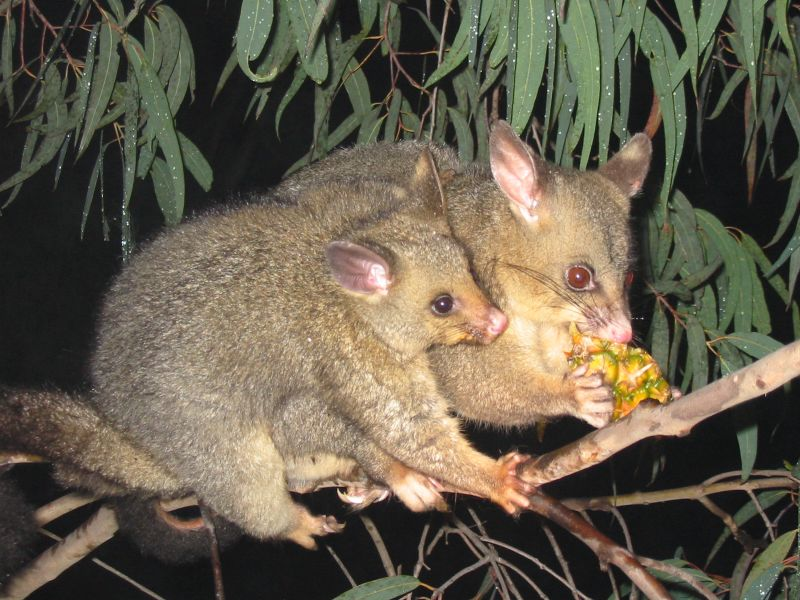
\includegraphics[height=2.8in]{ch1/possumPic/possumPic.jpg} \\
\begin{minipage}{\textwidth}
   \caption[possums]{The common brushtail possum of Australia\footnote{Photo by wollombi on Flickr: \texttt{http://flickr.com/photos/wollombi/58499575/}}.}
   \label{possumPic}
\end{minipage}
\end{center}
\end{figure}

Each row in the table represents a single possum or \term{case}\footnote{A case may also be called an \term{observational unit}.} and contains seven characteristics or measurements for that possum. For example, Possum 104 is a 3 year old female.

Each column of Table~\ref{possumDF} represents an attribute known about each case, and these attributes are called \term{variables}. For instance, the \var{age} variable holds the age of every possum in the data set. Descriptions of all seven {possum} variables are given below. % in Table~\ref{possumVariables}.
\begin{tabbing}
\hspace{\parindent}\= \var{pop}  \=\hspace{10mm}\=  location where possum was trapped (\resp{Vic} or \resp{other}) \\
\>\var{sex}  \>\>  possum's gender (\resp{m} or \resp{f}) \\
\>\var{age}  \>\>  age, in years (whole number, data range: \resp{1} to \resp{9}) \\
\>\var{headL}  \>\>  head length, in mm (data range: \resp{82.5} to \resp{103.1}) \\
\>\var{skullW}  \>\>  skull width, in mm (data range: \resp{50.0} to \resp{68.6}) \\
\>\var{totalL}  \>\>  total length, in cm (data range: \resp{75.0} to \resp{96.5}) \\
\>\var{tailL}  \>\>  tail length, in cm (data range: \resp{32.0} to \resp{43.0}) \\
\end{tabbing}
\addvspace{-5mm}
%%\begin{table}[ht]
%%\begin{center}\small
%%\begin{tabular}{l l}
%%\hline
%%{\bf variable} & {\bf description} \\
%%\hspace{0.5cm} \= \var{case}: ID number associated with the possum (\resp{1}, \resp{2}, ..., \resp{104}) \\
%%\> \var{site}: the location where each possum was trapped (\resp{1}, \resp{2}, ..., \resp{7}) \\
%%\hline
%\begin{itemize}
%\item[]\var{pop}: location where possum was trapped (\resp{Vic} or \resp{other})
%\item[]\var{sex}: possum's gender (\resp{m} or \resp{f})
%\item[]\var{age}: age, in years (whole number, data range: \resp{1} to \resp{9})
%\item[]\var{headL}: head length, in mm (data range: \resp{82.5} to \resp{103.1})
%\item[]\var{skullW}: skull width, in mm (data range: \resp{50.0} to \resp{68.6})
%\item[]\var{totalL}: total length, in cm (data range: \resp{75.0} to \resp{96.5})
%\item[]\var{tailL}: tail length, in cm (data range: \resp{32.0} to \resp{43.0})
%\end{itemize}
%%\> \var{earConch}: 
%%\hline
%%\end{tabular}
%%\end{center}
%%\caption{Variables and their descriptions for the \data{possum} data set.}
%%\label{possumVariables}
%%\end{table}

In practice, it is especially important to ask clarifying questions to ensure important aspects of the data are understood. For instance, the \term{levels} of the \var{pop} variable are not straightforward, so we should inquire to their meaning: \resp{Vic} represents possums that were trapped in Victoria while \resp{other} represents possums trapped in New South Wales or Queensland.

\subsection{Data Matrix}

The data in Table~\ref{possumDF} represent a \term{data matrix}, %\footnote{In R, a data matrix is called a \term{data frame}.}
which is a common way to organize data. Each row of a data matrix represents a separate case and each column represents a variable.

A data matrix called \data{cars} is shown in Table~\vref{carsDF}. Cars 1, 2, and 54 are shown with six variables: \var{type}, \var{price}, \var{mpgCity}, \var{driveTrain}, \var{passengers}, and \var{weight}, summarized in Table~\ref{carsVariables}:
\begin{table}
\begin{center}
\begin{tabular}{c ccc ccc}
  \hline
 & type & price & mpgCity & driveTrain & passengers & weight \\
  \hline
\resp{1} & \resp{small} & \resp{15.9} & \resp{25} & \resp{front} &  \resp{5} & \resp{2705} \\
  \resp{2} & \resp{midsize} & \resp{33.9} & \resp{18} & \resp{front} &  \resp{5} & \resp{3560} \\
$\vdots$ & $\vdots$ & $\vdots$ & $\vdots$ & $\vdots$ & $\vdots$ & $\vdots$ \\
  \resp{54} & \resp{midsize} & \resp{26.7} & \resp{20} & \resp{front} &  \resp{5} & \resp{3245} \\
  \hline
\end{tabular}
\end{center}
\caption{The \data{cars} data matrix.}
\label{carsDF}
%\end{table}
%\begin{table}
\begin{center}\small
\begin{tabular}{lp{9.5cm}}
\hline
{\bf variable} & {\bf description} \\
\hline
%\begin{itemize}
\var{type} & car type (\resp{small}, \resp{midsize}, or \resp{large}) \\
\var{price} & the average purchase price of the vehicles in \$1000's (positive number) \\
\var{mpgCity} & rated city mileage in miles per gallon (positive number) \\
\var{driveTrain} & the drive train (\resp{front}, \resp{rear}, \resp{4WD}) \\
\var{passengers} & passenger capacity (positive whole number, taking values \resp{4}, \resp{5}, or \resp{6}) \\
\var{weight} & car weight in pounds (positive number) \\
%\end{itemize}
\hline
\end{tabular}
\end{center}
\caption{Variables and their descriptions for the \data{cars} data set.}
\label{carsVariables}
\end{table}

\subsection{Variable relationships}
\label{variableRelations}

Many analyses are motivated by a researcher looking for a relationship between two or more variables. A biologist studying possums may want to know answers to some of the following questions.
\begin{enumerate}
\item[(1)]\label{questionAboutPossumHeadLengthAndWidth} If a possum has a shorter-than-average head, will its skull width usually be smaller or larger than the average skull width? \label{possumHeadSizeQuestion}
\item[(2)]\label{maleOrFemalePossumsLonger} Will males or females, on average, be longer? \label{possibleCausationQuestionForPossums}
\item[(3)]\label{whichPopulationOfPossumWillBeLargerOnAverage} Which population of possum will be larger on average: Victoria or the other locations?
\item[(4)]\label{doesTheProportionOfMalesDifferBasedOnLocation} Does the proportion of males differ based on location, i.e. from Victoria to the other locations?
\end{enumerate}

